\documentclass[12pt]{article}
\usepackage[spanish]{babel}
\usepackage[a4paper, left=3cm, right=2.5cm, top=2cm, bottom=2cm]{geometry}
\usepackage{graphicx}
\usepackage{float}
\usepackage{listings}
\usepackage{xcolor}
\usepackage{tikz}
\usepackage{url}

\definecolor{codegreen}{rgb}{0,0.6,0}
\definecolor{codegray}{rgb}{0.5,0.5,0.5}
\definecolor{codepurple}{rgb}{0.58,0,0.82}
\definecolor{backcolour}{rgb}{0.95,0.95,0.92}


\lstdefinestyle{mystyle}{
	language=Matlab,
	backgroundcolor=\color{white}, % Fondo blanco
	basicstyle=\sffamily\footnotesize, % Fuente Arial más pequeña
	keywordstyle=\color[HTML]{0072BD}\bfseries, % Palabras clave en azul oscuro
	commentstyle=\color[HTML]{008000}\itshape, % Comentarios en verde
	stringstyle=\color[HTML]{A2142F}, % Cadenas en rojo
	numberstyle=\tiny\color{gray}, % Números de línea en gris
	numbers=left, % Números de línea a la izquierda
	numbersep=3pt, % Separación entre los números de línea y el código
	frame=single, % Marco alrededor del código
	rulecolor=\color{black!50}, % Color del marco
	breaklines=true, % Permitir saltos de línea
	tabsize=2, % Tamaño de los tabuladores
	showspaces=false, % No muestra los espacios
	showstringspaces=false, % No muestra los espacios en cadenas
}

\lstset{style=mystyle}

\title{SISTEMAS DE CONTROL I \\ Trabajo final integrador 
	\\ Sistema de control de temperatura para un CPU}

\author{Docentes:\\ AGUERO CLAUDIO (Titular) \\ PEDRONI JUAN PABLO (Adjunto)
	\\ Alumnos: \\ Bernaus Julieta, Campos Mariano}
	
\begin{document}
	
\maketitle

\begin{center}
	
\includegraphics[width=0.7\linewidth]{Imagenes/Informe}
\end{center}

\begin{abstract}
	Este proyecto tiene como objetivo diseñar e implementar un sistema de control a lazo cerrado para regular la temperatura de un CPU mediante el ajuste dinámico de la velocidad de un ventilador. El sistema busca mantener la temperatura dentro de límites seguros, optimizando el desempeño y la vida útil del CPU.
\end{abstract}\newpage

\tableofcontents \newpage

\section{Definición del problema}

	\subsection{Principio de funcionamiento del sistema}
	El sistema propuesto es un controlador a lazo cerrado para regular la temperatura de un CPU mediante el ajuste de la velocidad de un ventilador. El principio de funcionamiento se basa en la retroalimentación: se mide constantemente la temperatura del CPU, se compara con un valor deseado (setpoint), y se ajusta dinámicamente la velocidad del ventilador para mantener la temperatura en los límites establecidos.

	\subsection{Variable a controlar}
	La variable a controlar es la temperatura del CPU,($T_{CPU}$ en grados Celsius, °C). El objetivo es mantenerla dentro de un rango seguro para evitar el sobrecalentamiento, con un setpoint ajustable dependiendo de la carga del sistema.
	
	\subsection{Medición de la variable de salida}
	Si bien algunos CPU tienen incorporados sensores de temperaturas internos,para nuestro caso utilizamos un sensor de temperatura LM35.
	
	\begin{itemize}
		\item Sensor:precisión de ±0.5°C.
		\item Acondicionamiento de señal:El LM35 podría requerir un ADC si fuera necesario utiliza un microcontrolador (Se determina en las secciones posteriores).
	\end{itemize}
	
	
	
	\subsection{Ejecución de la acción de control}
	La acción de control se ejecutará mediante un ventilador de corriente continua (DC) cuyo motor será controlado con señales PWM (modulación por ancho de pulso). La señal PWM ajustará las revoluciones por minuto (RPM) del ventilador, proporcionalmente a la señal de control generada por el comparador.
	
	
	\subsection{Variables del sistema}
	\begin{table}[h!]
		\centering
		\begin{tabular}{|c|c|l|}
			\hline
			\textbf{Variable} & \textbf{Unidad} & \textbf{Descripción} \\ \hline
			$T_{CPU}$ & °C & Temperatura del CPU. \\ \hline
			$V_{Fan}$ & RPM & Velocidad del ventilador. \\ \hline
			Señal de control (u) & \% (Duty Cycle) & Señal generada por el controlador (PWM). \\ \hline
			$T_{Amb}$ & °C & Temperatura ambiente (perturbación). \\ \hline
		\end{tabular}
		\caption{Variables del sistema con sus unidades y descripciones.}
		\label{tab:variables}
	\end{table}
	
	
	\subsection{Posibles perturbaciones}
	\begin{itemize}
		\item Variaciones en la temperatura ambiente $T_{Amb}$ El sistema debe compensar los cambios en la temperatura externa.
		\item Carga del CPU: A mayor carga, se genera más calor, lo que afecta directamente la variable controlada, la $T_{CPU}$.
		\item Fluctuaciones de voltaje en el suministro eléctrico: Pueden alterar el funcionamiento del ventilador(No se tiene en cuenta para el diseño).
	\end{itemize}
	
	\subsection{No linealidades involucradas}
	El sistema de control que regula la temperatura del CPU a través del ventilador debe abordar múltiples fuentes de no linealidad:
	
	\begin{itemize}
		\item Ventilador: La relación entre el ciclo de trabajo PWM y la velocidad del ventilador es no lineal, especialmente a bajas RPM.
		\item Sensores de temperatura: Los sensores tienen respuestas no lineales que deben ser compensadas para obtener mediciones precisas.
		\item Transferencia de calor: El comportamiento térmico del CPU y su interacción con el sistema de enfriamiento (ventilador) es no lineal.
	\end{itemize}
	
	\subsection{Niveles de señal de entrada y salida}
	Existen dos principales señales, donde es de especial interés conocer sus rangos dinámicos, la  $T_{CPU}$ y por otro lado la señal de control $PWM$.Respecto a la primer señal tenemos que la temperatura máxima que puede alcanzar un CPU depende de varios factores, como el modelo específico del procesador, el sistema de refrigeración utilizado, y las condiciones ambientales.Se debe tener en cuenta que:
	
	\begin{itemize}
		\item Temperatura nominal de operación: Un CPU típico a máxima carga generalmente puede alcanzar temperaturas entre 70°C y 90°C. Este rango depende del tipo de CPU (por ejemplo, Intel o AMD), el proceso de fabricación, y las condiciones de refrigeración.
		\item Temperatura crítica o límite superior: Los fabricantes de CPUs suelen establecer una temperatura máxima segura alrededor de los 100°C a 105°C. Si el CPU alcanza estas temperaturas, el sistema activará medidas de protección, como el thermal throttling (reducción de la velocidad de reloj) o el apagado del sistema para evitar daños.
	\end{itemize}
	
	De lo mencionado anteriormente se concluye que la $T_{CPU}$ oscila entre 30°C  y 100°C, y por tanto teniendo en cuenta el datasheet del sensor LM35, el rango dinámico de la señal resulta de $300[mV]$ hasta $1[V]$.
	Para la segunda señal de interés tenemos la señal PWM, esta varia segun el ciclo de trabajo desde 0\% hasta el 100\%, esto se traduce en un rango dinámico de $0[V]$ hasta $5[V]$(5000[RPM]).
	 
\section{Análisis de la planta}
	 En este caso la planta es el CPU con su  disipador, para obtener el modelo matemático se recurre a la ley de Ohm térmica,la inercia térmica de los cuerpos (CPU y disipador) se modela como una capacidad, se tiene:
	 \begin{equation}
	 	I[A]=\frac{\bigtriangleup V[V]}{R[ohm]}=Q[W]=\frac{\bigtriangleup T[Cº]}{Rth[Cº/W]}
	 \end{equation}
	 
	 \begin{equation}
	 	Cth[J/C]
	 \end{equation}\newpage
	 
	 \begin{figure}[h!]
	 	\centering
	 	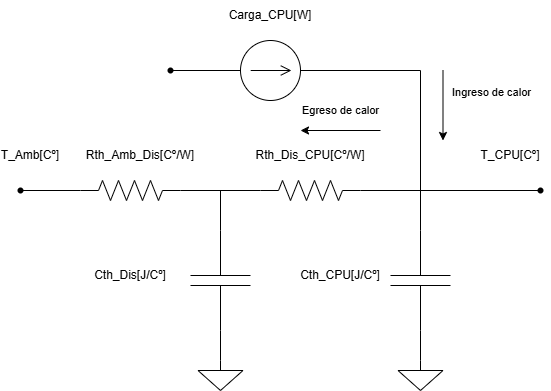
\includegraphics[width=0.7\linewidth]{Imagenes/Modelo_planta}
	 	\caption[Modelo de la planta]{Modelo de la planta}
	 	\label{fig:modeloplanta}
	 \end{figure}
	 
	 Para la perturbación producida por la carga del CPU, esta aporta una cantidad de calor $Q$ a la planta, por lo que se puede modelar con una fuente de corriente.Como resultado del modelo tenemos dos flujos de calor, el entrante por la carga del CPU y el saliente debido a que $T_{Amb}<T_{CPU}$.Se calcula la función de transferencia, con el siguiente código de Matlab:
	
	\begin{lstlisting}
		% Declarar variables simbolicas
		syms T_Amb T_CPU T_Dis 
		syms Rth_Amb_Dis Rth_Dis_CPU Cth_Dis Cth_CPU
		syms s
		
		% Temperaturas y flujo de calor
		% Primera etapa: T_Amb -> T_Dis
		Q1 = (T_Amb - T_Dis) / Rth_Amb_Dis; % Flujo de calor a traves de Rth_Amb_Dis
		eq1 = Q1 == Cth_Dis * s * T_Dis;   % Relacion por la capacidad termica
		
		% Segunda etapa: T_Dis -> T_CPU
		Q2 = (T_Dis - T_CPU) / Rth_Dis_CPU; % Flujo de calor a traves de Rth_Dis_CPU
		eq2 = Q2 == Cth_CPU * s * T_CPU;    % Relacion por la capacidad termica
		
		% Resolver el sistema de ecuaciones
		% Se despeja T_Dis y T_CPU en terminos de T_Amb
		sol = solve([eq1, eq2], [T_Dis, T_CPU]);
		
		% Obtener T_CPU como funcion de T_Amb
		T_CPU_T_Amb = collect(simplify(sol.T_CPU / T_Amb),s)
		
		Rth_Amb_Dis = 0.5;    % Resistencia  termica entre T_Amb y T_Dis [C/W]
		Rth_Dis_CPU = 0.3;    % Resistencia  termica entre T_Dis y T_CPU [C/W]
		Cth_Dis = 10;         % Capacitancia termica en el nodo T_Dis [J/C]
		Cth_CPU = 5;          % Capacitancia termica en el nodo T_CPU [J/C]
		
		T_CPU_T_Amb=eval(T_CPU_T_Amb)
	\end{lstlisting}
	
	Como resultado del análisis de obtenemos:
	\begin{equation}
		FdT_{Planta}=\frac{T_{CPU}(s)}{T_{Amb}(s)}=\frac{1}{7.5s^2+6.5s+1}
	\end{equation}
	
	
	 \subsection{Diagrama de bloques del sistema}
	 Se plantea un diagrama de bloques para modelar el sistema en su totalidad, se identifican sus partes principales(comparador, planta, sensor), las variables de entrada, salida y perturbaciones, ademas se detalla como interactúan estas entre si.
	 \begin{itemize}
	 	\item Entrada (señal de referencia):La temperatura deseada o setpoint (se puede suponer una temperatura objetivo o de referencia a mantener para el CPU, $T_{ref}$.
	 	
	 	\item Comparador:Compara la temperatura medida con la de referencia y genera una señal de control en forma de PWM para el ventilador.
	 	
	 	\item Actuador: Recibe la señal PWM del comparador y ajusta su velocidad.
	 	
	 	\item Perturbaciones:La carga del CPU es la principal perturbación que afecta la variable de salida.
	 	
	 	\item Sensor:Mide la temperatura real del CPU, $T_{CPU}$ y esta señal es retroalimentada al comparador.
	 	
	 	\item Planta: El CPU es el elemento a controlar, las variables de entrada son las perturbaciones que afectan su temperatura, y la refrigeración qu aporta el ventilador, la salida es el processvalue $T_{CPU}$
	 \end{itemize}
	 
	\begin{figure}[h!]
		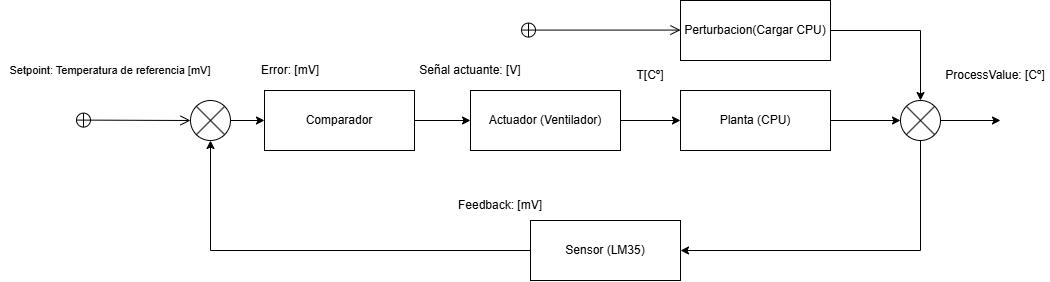
\includegraphics[width=1\linewidth]{Imagenes/Sistema_comleto}
		\caption[Sistema completo]{Sistema completo}
		\label{fig:sistemacomleto}
	\end{figure}
	
	\subsection{Modelado matemático de los componentes}
	
		\subsubsection{Sensor de temperatura}
		En el caso de la función de transferencia del sensor de temperatura LM35,esta se puede obtener de forma teórica, ya que en el datasheet se encuentra la expresión $V_{OUT}=F(T_{Amb})$, para la aplicación típica (FIGURE 1. Basic Centigrade Temperature Sensor), la expresión resulta:
		
		\begin{equation}
			V_{OUT}[V]= 0[V]+0.01[V].T_{Amb}[°C]
		\end{equation}
		
		La función de transferencia de interés, se obtienen pasando la ecuación al dominio operacional y despejando la expresión $Voltaje/Temperatura$, esta resulta:
		
		\begin{equation}
			FdT_{Sensor}=\frac{V_{LM35}(s)}{T_{CPU}(s)}=0.01
		\end{equation}
		
		\subsubsection{Ventilador}
		Para obtener la función de transferencia del ventilador se opto por hacerlo de forma experimental, ya que la relación entrada-salida de la señal PWM y temperatura, no se encontraba disponible en ninguna bibliografía.El procedimiento es el siguiente:
		
		\begin{itemize}
			\item Armar el sistema de refrigeración con el ventilador y el habitáculo donde se va a encontrar el CPU.
			\item Hacer variar la señal de entrada PWM del ventilador y medir la temperatura resultante en el habitáculo.
			\item Con los datos obtenidos, mediante un script en Matlab, obtener la función de transferencia
		\end{itemize}
		
		Nota: En nuestro caso los datos son simulados con un script de Python.
		
		\begin{figure}[h!]
			\label{fig:pwmvstemp}
			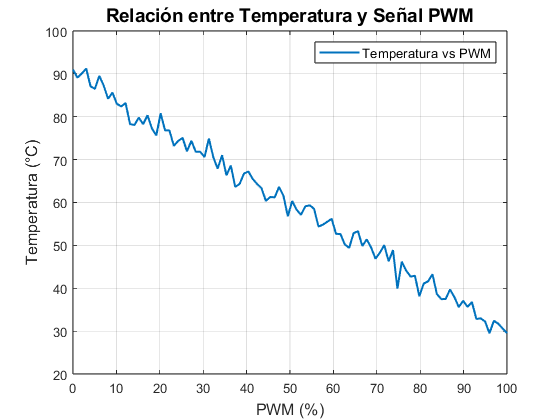
\includegraphics[width=1\linewidth]{Imagenes/pwm_vs_temp}
			\caption[Datos recopilados]{Datos recopilados}
		\end{figure}\newpage
		
		Con los datos obtenidos se realiza el siguiente análisis para obtener la función de transferencia:
		
		\begin{lstlisting}
			%Calculo de funcion de transferencias para el vantilador
			%Importamos los datos obtenidos de las mediciones
			opts = delimitedTextImportOptions("NumVariables", 2);
			opts.DataLines = [2, Inf];
			opts.Delimiter = ",";
			opts.VariableNames = ["PWM", "TemperatureC"];
			opts.VariableTypes = ["double", "double"];
			opts.ExtraColumnsRule = "ignore";
			opts.EmptyLineRule = "read";
			
			% Leer el archivo CSV como tabla
			data = readtable("D:\GD\Sistemas de control I\Trabajo-Integrador-SCI\Datos\pwm_temperature_data.csv",opts);
			
			% Separar las columnas en variables
			PWM = data.("PWM"); % Columna PWM
			Temperature = data.("TemperatureC"); % Columna Temperatura
			
			% Crear el grafico
			figure;
			plot(PWM, Temperature, 'LineWidth', 1.5, 'MarkerSize', 6, 'DisplayName', 'Temperatura vs PWM');
			grid on;
			xlabel('PWM (%)', 'FontSize', 12);
			ylabel('Temperatura (C)', 'FontSize', 12);
			title('Relacion entre Temperatura y Senal PWM', 'FontSize', 14);
			legend('show', 'Location', 'northeast', 'FontSize', 10);
			
			
			% Crear entrada y salida como senales en tiempo (asumiendo un muestreo uniforme)
			t = linspace(0, length(PWM)-1, length(PWM)); % Tiempo ficticio
			u = PWM; %Entrada (PWM )
			y = Temperature; % Salida (Temperatura)
			
			% Ajustar un modelo de primer o segundo orden (dominio Laplace)
			data_id = iddata(y, u, 1); % Crear datos de identificacion con un muestreo ficticio de 1s
			model = tfest(data_id, 1, 0); % Ajustar un modelo de primer orden sin ceros
			
			% Mostrar la funcion de transferencia estimada
			disp('Funcion de transferencia estimada:');
			disp(model);
			
			% Graficar comparacion entre el modelo ajustado y los datos
			figure;
			compare(data_id, model);
			title('Comparacion entre datos reales y modelo ajustado', 'FontSize', 14);
			xlabel('Tiempo (s)', 'FontSize', 12);
			ylabel('Temperatura (C)', 'FontSize', 12);
			legend('Datos reales', 'Modelo ajustado', 'Location', 'best', 'FontSize', 10);
			grid on;
		\end{lstlisting}
		
		La función de transferencia obtenida resulta:
		\begin{equation}
			FdT_{Ventilador}=\frac{T_{Amb}(s)}{PWM(s)}=\frac{-0.0038}{s+0.007}
		\end{equation}
		
		\begin{figure}[h!]
			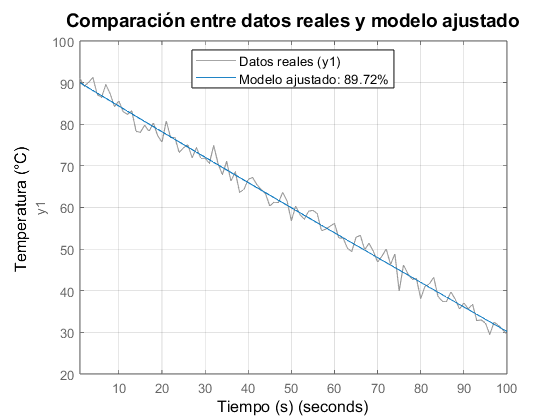
\includegraphics{Imagenes/Ajuste_modelo}
			\caption[Ajuste del modelo]{Ajuste del modelo}
			\label{fig:ajustemodelo}
		\end{figure}
	
		\subsubsection{Comparador}
		Para obtener la función de transferencia del comparador suponemos una $V_{ref}=600[mV]$, esta se condice con una temperatura de 60 ºC, la señal de entrada va ser el error que resulta de la resta $V_{ref}-V_{LM35}$, en el caso de que el error sea $0[V]$ la salida de PWM al ventilador es cero, esto significa que esta operando a una temperatura segura, para el caso donde el error sea $-300[mV]$ esto quiere decir que la temperatura del CPU ronda los 90 ºC, la salida PWM debe ser $5[V]$, entre medio de estos dos valores definimos una variación lineal, para errores positivos la salida de PWM también debe ser $0[V]$ esto significa que esta por debajo de los 60 ºC, con este análisis calculamos una recta que pase por estos dos puntos, para luego calcular la función de transferencia.\newpage
	
		\begin{lstlisting}
			% Parametros iniciales
			V_ref = 0.6; % [V] Referencia de temperatura (60 C)
			V_LM35_safe = V_ref; % Valor seguro donde el error es 0 [V]
			V_LM35_danger = 0.3; % [V] (90 C -> 600 - 300 = -0.3 [V])
			
			% Valores de PWM en los puntos limite
			PWM_safe = 0; % PWM = 0 [V] (Temperatura segura)
			PWM_danger = 5; % PWM = 5 [V] (Temperatura alta)
			
			% Calculo de la pendiente de la recta
			% Recta entre los puntos: (-0.3, 5) y (0, 0)
			m = (PWM_danger - PWM_safe) / (V_LM35_safe - V_LM35_danger);
			
			% Ordenada al origen de la recta
			b = PWM_safe - m * (V_LM35_safe - V_ref);
			
			% Mostramos la funcion lineal calculada
			fprintf('La funcion PWM respecto al error (V_ref - V_LM35) es:\n');
			fprintf('PWM = %.2f * error + %.2f\n', m, b);
			
			% Crear el modelo de funcion de transferencia
			% Supongamos entrada U(s) (error) y salida Y(s) (PWM)
			% Relacion directa en dominio del tiempo: PWM = m * error + b
			numerator = [m]; % Numerador (ganancia m)
			denominator = [1]; % Denominador (sistema de primer orden, estatico)
			sys = tf(numerator, denominator);
			
			% Visualizar la respuesta del sistema
			% Definir un rango de errores desde -300 mV a +300 mV
			error = linspace(-0.3, 0.3, 100); % [V]
			PWM = m * error + b;
			
			% Forzar PWM a ser cero para errores positivos
			PWM(error > 0) = 0;
			
			% Graficar
			figure;
			plot(error * 1000, PWM);
			grid on;
			xlabel('Error [mV]');
			ylabel('Salida PWM [V]');
			title('Relacion entre Error y PWM');
			legend('PWM vs Error');
			
		\end{lstlisting}
		La la ecuación de la recta es:
		\begin{equation}
			PWM[V]=16.67Error[V]-0
		\end{equation}
		
		La función de transferencia es simplemente la pendiente. Esto representa una ganancia constante entre el error y la señal PWM de salida.Notar que la función de transferencia solo captura las dependencias entre la salida y la entrada. Los términos independientes (constantes) no afectan la relación entre la entrada y la salida en términos de función de transferencia.
		El resultado del análisis anterior es:
		
		\begin{equation}
			FdT_{Comparador}=\frac{PWM(s)}{Error(s)}=16.67
		\end{equation}\newpage

	\subsection{Función de transferencia global}
	Con todos los elementos del sistema modelados calculamos la función de transferencia global, la obtención de esta se realiza mediante el álgebra de bloques con el siguiente script de matlab:
	
	\begin{figure}[h!]
		\centering
		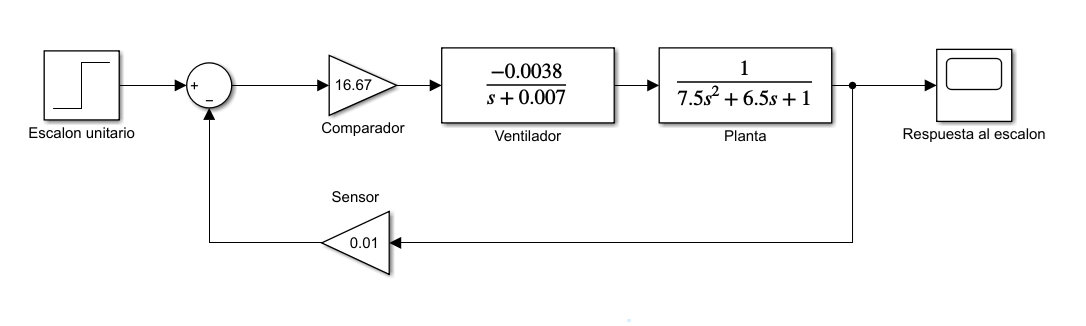
\includegraphics[width=1\linewidth]{Imagenes/Simulink}
		\caption[Diagrama de bloques del sistema]{Diagrama de bloques del sistema}
		\label{fig:simulink}
	\end{figure}
	
	\begin{lstlisting}
		% Definir la variable simbolica para la funcion de transferencia
		s = tf('s');
		
		% Funciones de transferencia individuales
		FdT_Planta = 1/(7.5*s^2 + 6.5*s + 1);         % Funcion de transferencia de la planta
		FdT_Sensor = 0.01;                            % Funcion de transferencia del sensor
		FdT_Ventilador = -0.0038/(s + 0.007);         % Funcion de transferencia del ventilador
		FdT_Comparador = 16.67;                       % Funcion de transferencia del comparador
		
		%Utilizando el algebra de bloques obtenemos la fdt global
		G=FdT_Planta*FdT_Ventilador*FdT_Comparador;
		H=FdT_Sensor;
		
		%Funcion de transferencia global
		FdT_Global=feedback(G,H);
		
		% Funcion de transferencia global original
		disp('La funcion de transferencia global original es:');
		FdT_Global  
	\end{lstlisting}
	
	La función de transferencia global resulta:
	\begin{equation}
		FdT{Global} =\frac{-0.06335}{7.5 s^3+6.553 s^2+1.046s+0.006367}
	\end{equation}
	
	\subsection{Análisis de estabilidad absoluta y relativa}
	Para probar la estabilidad absoluta de una función de transferencia, se puede analizar los polos de la misma. Un sistema es estable de forma absoluta si todos sus polos tienen partes reales negativas. Esto implica que, para que el sistema sea estable, la solución a la ecuación característica asociada a la función de transferencia debe tener raíces con partes reales negativas.Por otro lado valuamos la estabilidad relativa de sistema con herramientas gráficas como el lugar de raíces, que muestra cómo evolucionan las posiciones de los polos a lazo cerrado cuando varia el valor de kp.
	
	\begin{lstlisting}
		% Definir la funcion de transferencia a lazo abireto (GH)
		GH = FdT_Comparador*FdT_Ventilador*FdT_Planta*FdT_Sensor
		
		% Calcular y mostrar los ceros de la funcion de transferencia a lazo abierto
		disp('Ceros de la funcion de transferencia:');
		zero_GH = zero(GH);
		disp(zero_GH);
		
		% Calcular y mostrar los polos de la funcion de transferencia a lazo abierto
		disp('Polos de la funcion de transferencia:');
		pole_GH = pole(GH);
		disp(pole_GH);
		
		% Graficar el lugar de raices de la funcion de transferencia
		figure;
		rlocus(GH);
		grid on;
		
		%El sistema es marginalmente estable, para k<11
		rlocfind(GH);
		grid on;
		
		title('Lugar de Raices de la Funcion de Transferencia');
		xlabel('Parte Real');
		ylabel('Parte Imaginaria');
	\end{lstlisting} 
	
	Las raíces de la ecuación característica son:
	\begin{equation}
		P1=-0.6667   ,P2=-0.2000	,P3=-0.0070
	\end{equation}
	
	Todas las raíces de la ecuación característica tienen parte real negativa, podría decirse que el sistema es estable de forma absoluta, de forma relativa podemos decir que  para valores de k menores a 11 el sistema es estable y para valores mayores el  deja de serlo.\newpage
	  
	\begin{figure}
		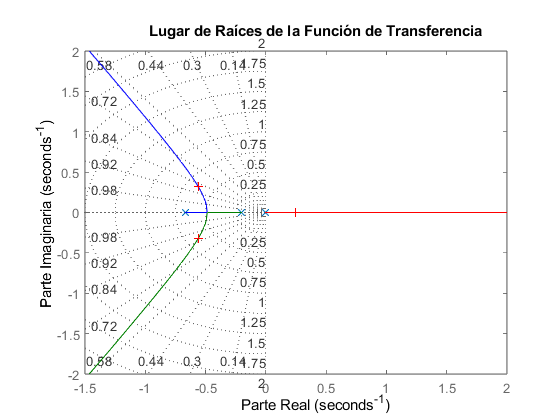
\includegraphics[width=1\linewidth]{Imagenes/Rlocus}
		\caption[Lugar de raíces de la función de transferencia global]{Lugar de raíces de FdTGlobal}
		\label{fig:rlocus}
	\end{figure}
	
	\subsection{Análisis de la respuesta temporal}
	Verificamos el comportamiento del sistema, simulando la respuesta al escalón unitario con distintos valores de kp, la forma de respuesta es decreciente esto se debe a que aumenta la señal de entrada disminuye la salida (ganancia negativa) este comportamiento es esperable ya que la temperatura debe disminuir cuando la señal de control (PWM) aumenta.
	
	\begin{lstlisting}
		%Definimos distintos valores de k para simular la respuesta 
		k1 = 5;
		k2 = 20;
		
		%Por la ubicacion del polo dominante resulta imposible una compensacion
		%solo proporcional ya que el polo dominante esta muy cerca del origen y
		%hace al sistema muy lento
		
		% Crear un figure con tres subplots
		figure;
		
		% Primer subplot: Respuesta para k1
		subplot(2, 1, 1);
		step(feedback(k1*G,H));
		title('kp1=5 "Estable"');
		xlabel('Time')
		ylabel('Amplitude')
		grid on;
		
		% Segundo subplot: Respuesta para k2
		subplot(2, 1, 2);
		step(feedback(k2*G,H));
		title('kp2=20 "Inestable"');
		xlabel('Time')
		ylabel('Amplitude')
		grid on;
		
		figure;
		step(feedback(G,H));
		title('Respuesta temporal sin kp');
		xlabel('Time')
		ylabel('Amplitude')
		grid on
	\end{lstlisting}
	
	En el resultado de la simulación podemos ver que el sistema es estable para $kp=5$ e inestable para $kp=20$, este resultado es esperable de acuerdo al análisis de estabilidad relativa que se realizo anteriormente.
	
	\begin{figure}[bh]
		\centering
		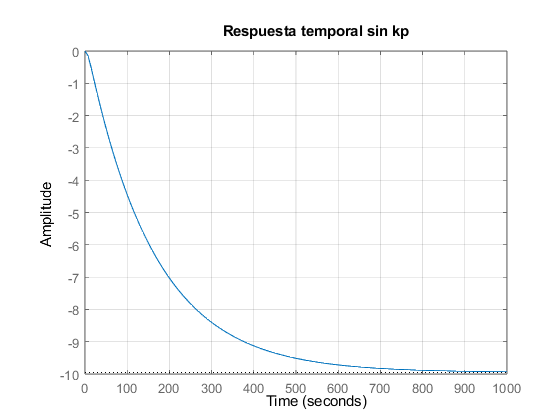
\includegraphics[width=1\linewidth]{Imagenes/Respuesta_temporal_sin_kp}
		\caption[Respuesta temporal sin compensación proporcional]{Respuesta temporal sin compensación proporcional}
		\label{fig:respuestatemporalsinkp}
	\end{figure}
	
	\begin{figure}
		\centering
		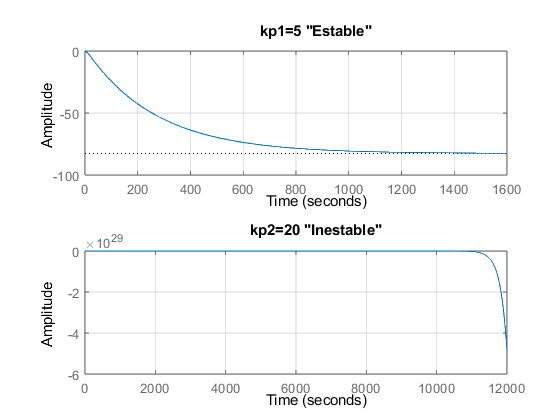
\includegraphics[width=1\linewidth]{Imagenes/Respuesta_escalon_Fdtglobal}
		\caption[Respuesta al escalo unitario]{Respuesta al escalo unitario}
		\label{fig:respuestaescalonfdtglobal}
	\end{figure}\newpage
	
	\subsubsection{Determinación del tipo de sistema}
	Para determinar el tipo de sistema, nos enfocamos en la cantidad de integradores en la trayectoria directa, lo cual se observa en la cantidad de polos en el origen (s = 0) de la función de transferencia a lazo abierto.	En este caso, la función de transferencia no tiene ningún factor 's' aislado en el denominador.Por lo tanto, este sistema es de Tipo 0. Esto quiere decir que el error de estado estable para una entrada escalón es constante, en nuestro caso esta representa la temperatura de referencia (setpoint), por lo que resulta de interés tener el menor error de estado estable posible.

	\subsubsection{Polos dominantes}
	Respecto a los polos dominantes, en este caso lo tenemos en $p3=-0.007$, su proximidad al origen hace que la respuesta del sistema sea demasiada lenta (esto es esperable en sistemas térmicos), podemos ver en la respuesta temporal que el tiempo de establecimiento esta en el orden de los 700 segundos, este valor dista mucho de las especificaciones de diseño por lo que resulta imperioso corregirlo al momento de compensar el sistema.\newpage
	
\section{Especificaciones de diseño}
	Partimos de las especificaciones de diseño en el dominio del tiempo, los requerimientos son:
	\begin{equation}
		ess=min
	\end{equation}
	\begin{equation}
		ts\leq 50[s]
	\end{equation}
	\begin{equation}
		Mp\leq 4 \%
	\end{equation}
	
	Para un primer análisis, podríamos tratar de implementar un compensador PID que cancele los dos polos dominantes $p2=-0.2$ y $p3=-0.007$, esto permite mejorar la respuesta temporal (hacerlo mas rápido al sistema) y al mismo tiempo mejorar el error de estado estable (aumenta el tipo), ambas cosas son deseables, sin embargo el hecho de que el sistema tenga una ganancia negativa y un polo al origen, hace que el sistema compensado sea inestable para todo kp, como se muestra en el siguiente análisis.
	
\section{Diseño del controlador}
	Análisis para la implementación de para el compensador:
	\begin{lstlisting}
		% Definir la variable simbolica para la funcion de transferencia
		s = tf('s');  
		
		% Funciones de transferencia individuales
		FdT_Planta = 1/(7.5*s^2 + 6.5*s + 1);         % Funcion de transferencia de la planta
		FdT_Sensor = 0.01;                            % Funcion de transferencia del sensor
		FdT_Ventilador = -0.0038/(s + 0.007);         % Funcion de transferencia del ventilador
		FdT_Comparador = 16.67;                       % Funcion de transferencia del comparador
		
		% Definir la funcion de transferencia a lazo abierto (GH)
		G=FdT_Planta*FdT_Ventilador*FdT_Comparador;
		H=FdT_Sensor;
		disp('La funcion de transferencia a lazo abierto "GH"');
		GH=G*H
		
		% Mostrar la funcion de transferencia a lazo abierto en forma de ceros y polos
		disp('La funcion de transferencia a lazo abierto explicita');
		GH=zpk(GH)  
		
		% La ecuacion caracteristica de la funcion de transferencia a lazo abierto resulta ser:
		% Ec(s) = (s+0.6667)(s^2 + 0.207s + 0.0014)
	\end{lstlisting}\newpage
	
	Para cancelación de polos dominantes con PID tenemos:
	\begin{lstlisting}
		% La forma del PID es: PID = kp * (Ti*Td*s^2 + Ti*s + 1) / (Ti*s)
		
		% Vamos a igualar terminos con la ecuacion de segundo orden en el denominador
		
		% Comparacion con la ecuacion de segundo orden:
		% a^2 + b*s + c = s^2 + 0.207*s + 0.0014
		
		c = 1;               % Valor de c (termino constante)
		b = 0.207/0.0014;    % Calculamos b
		a = 1/0.0014;        % Calculamos a
		
		Ti = b              
		Td = a/Ti        
		
		% Armamos el controlador PID utilizando los valores de Ti y Td
		PID =(Ti*Td*s^2 +Ti*s+1)/(Ti*s) 
		
		% Armamos la funcion de transferencia a lazo abierto compensado (con PID)
		FdT_Global_PID = PID*GH
		
		% Verificamos la cancelacion de polos
		figure;
		subplot(2,1,1);                  % Primer subplot para la funcion a lazo abierto
		pzmap(GH);       % Muestra el mapa de polos y ceros de la funcion a lazo abierto
		title('Mapa de Polos y Ceros a lazo abierto "GH"');
		xlabel('real');
		ylabel('imaginaria');
		grid on;
		
		subplot(2,1,2);          % Segundo subplot para la funcion con PID
		pzmap(FdT_Global_PID);  % Muestra el mapa de polos y ceros de la funcion compensada
		title('Mapa de Polos y Ceros con Controlador PID');
		xlabel('real');
		ylabel('imaginaria');
		grid on;      
		
		% Simplificamos la expresion para obtener una forma mas compacta
		FdT_Global_PID = minreal(FdT_Global_PID)  % Simplificacion de la fdt
		figure;
		rlocus(FdT_Global_PID);         
		grid on;                          
		title('Lugar de raices de la funcion de transferencia compensada');
	\end{lstlisting}
	
	La función de transferencia del controlador PID resulta:
	\begin{equation}
		PID(s)=\frac{714.3s^2 + 147.9s + 1}{147.9s}
	\end{equation}
	
	La función a lazo cerrado global compensada es:
	\begin{equation}
		FdT_{GlobalComp}=\frac{0.4525s^2 + 0.09366s + 0.006335}{1109s^4 + 968.8s^3 + 154.6s^2 + 1.035s}
	\end{equation} 
	
	En este grafico se verifica la cancelación de los dos polos mas dominantes y el polo al origen que se agrega por el PID.
	\begin{figure}[h!]
		\centering
		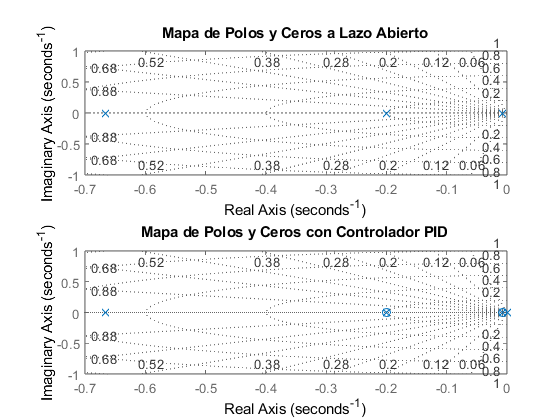
\includegraphics[width=1\linewidth]{Imagenes/Pzmap}
		\caption[Polos y ceros, antes vs después de la compensación]{Polos y ceros, antes vs despues de la compensación}
		\label{fig:pzmap}
	\end{figure}
	
	El lugar de raíces confirma que el sistema termina siendo inestable para todo kp,esto también descarta el compensador PI, por lo mencionado anteriormente ,la única opción radica en un compensador PD, el cual lo desarrollamos a continuación.\newline
	
	Otra  alternativa seria añadir un inversor, para que la ganancia total del sistema resulte positiva y poder utilizar el compensador PID,para mejorar tanto la respuesta transitoria como el error en estado estable del sistema.\newpage
	  
	\begin{figure}[bht]
		\centering
		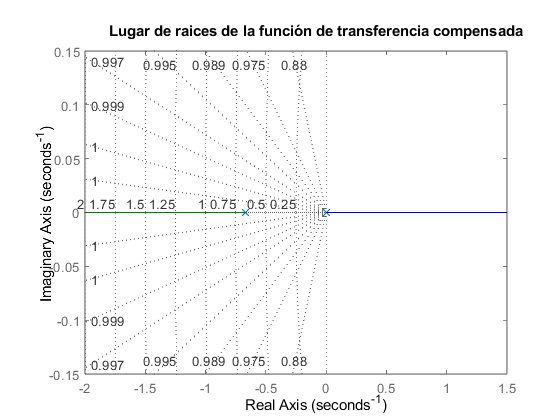
\includegraphics[width=1\linewidth]{Imagenes/Rlocus_comp_PID}
		\caption[Lugar de raíces FdT compensado por PID]{Lugar de raíces FdT compensado por PID}
		\label{fig:rlocuscomppid}
	\end{figure}
	
	Para el compensador PD tenemos:
	\begin{lstlisting}
		% La forma del PI es: PID = kpTd(s+1/Td)
		
		% Teniendo en cuenta que el polo dominante es s=-0.007 tenemos:
		Td=1/0.007
		
		% Armamos el controlador PI utilizando los valores de Ti
		PD = Td*(s+1/Td)
		
		% Armamos la funcion de transferencia a lazo abierto compensado (con PD)
		FdT_Global_PD = PD*GH
		
		% Verificamos la cancelacion de polos
		figure;
		subplot(2,1,1);                  % Primer subplot para la funcion a lazo abierto
		pzmap(GH);       % Muestra el mapa de polos y ceros de la funcion a lazo abierto
		title('Mapa de Polos y Ceros a lazo abierto "GH"');
		xlabel('real');
		ylabel('imaginaria');
		grid on;
		
		subplot(2,1,2);          % Segundo subplot para la funcion con PI
		pzmap(FdT_Global_PD);  % Muestra el mapa de polos y ceros de la funcion compensada
		title('Mapa de Polos y Ceros con Controlador PD');
		xlabel('real');
		ylabel('imaginaria');
		grid on;
		
		% Simplificamos la expresion para obtener una forma mas compacta
		FdT_Global_PD = minreal(FdT_Global_PD)  % Simplificacion de la fdt
		
		figure;
		rlocus(FdT_Global_PD);         
		grid on;                         
		title('Lugar de raices de la funcion de transferencia compensada');
		
		%Estable para kp<11
		rlocfind(FdT_Global_PD);
		grid on;
	\end{lstlisting}
	
	La función de transferencia del controlador PD resulta:
	\begin{equation}
		PD(s)=142.9s+1
	\end{equation}
	
	La función a lazo cerrado global compensada es:
	\begin{equation}
		FdT_{GlobalComp}=\frac{-0.0120}{s^2+0,8667s+0,1333}
	\end{equation}
	
	Verificamos la cancelación de polos dominantes y buscamos un valor de kp que verifique los requerimientos.
	\begin{figure}[h!]
		\centering
		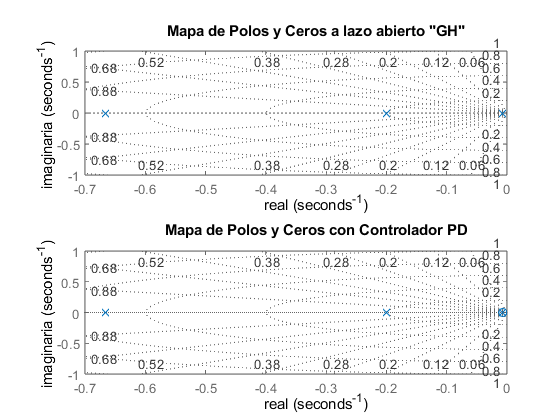
\includegraphics[width=1\linewidth]{Imagenes/Pzmap_PD}
		\caption[Cancelación de polos dominantes PD]{Cancelación de polos dominantes PD}
		\label{fig:pzmappd}
	\end{figure}\newpage
	
	\begin{figure}
		\centering
		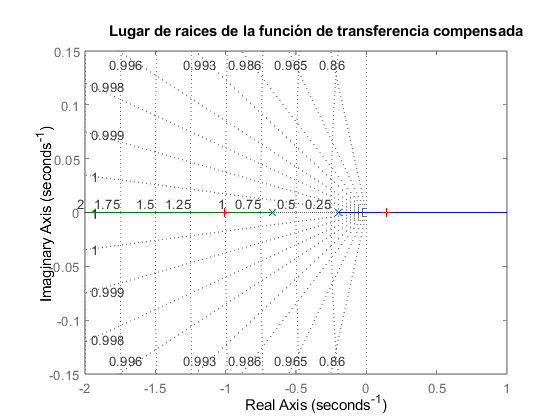
\includegraphics[width=1\linewidth]{Imagenes/Rlocus_comp_PD}
		\caption[Lugar de raíces compensador PD]{Lugar de raíces compensador PD}
		\label{fig:rlocuscomppd}
	\end{figure}
	
	Analizando el lugar de raíces podemos concluir que el sistema es estable para todo $kp<11$, a menor el valor de este, mayor velocidad de respuesta se obtiene.Un valor adecuado de ganancia proporcional es $kp=1$ ya que cumple con el tiempo de establecimiento que se tiene como requerimiento

\section{Simulación}
	En esta sección nos interesa compara la respuesta temporal antes y después de compensar, ademas de calcular el error de estado estable del sistema.
	
	\begin{lstlisting}
		% El valor que satisface los requerimientos es kp = 1
		figure;
		
		kp=1;
		step(feedback(G,H),feedback(kp*G*PD,H));
		grid on;
		
		title('Comparativa respuesta temporal');
		legend('no compensado', 'compensado')
		
	\end{lstlisting}\newpage
	
	\begin{figure}[h!]
		\centering
		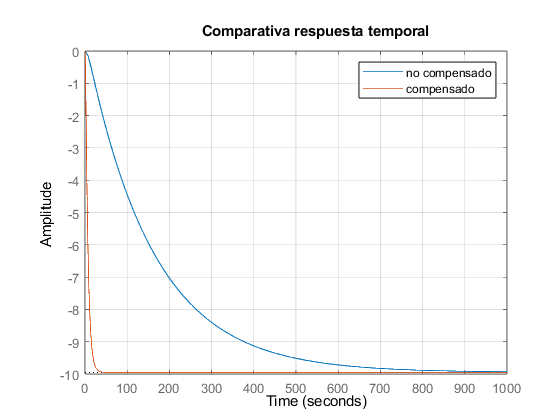
\includegraphics[width=1\linewidth]{Imagenes/Respuesta_temporal_comparativa}
		\caption[Respuesta temporal comparativa]{Respuesta temporal comparativa}
		\label{fig:respuestatemporalcomparativa}
	\end{figure}
	
	Se puede ver una mejora significativa en el tiempo de establecimiento.Respecto al error en estado estable podemos realizar el siguiente análisis, sabemos que el sistema no tiene polos en el origen (Tipo 0), por lo que esperamos un error de estado estable constante frente a la respuesta de un escalón, luego:
	
	\begin{lstlisting}
		%Analisis del error en estado estable, la fdt global resulta un sistema de
		%tipo 0, por lo tanto se espera que el error en estado estable sea
		%constante.
		
		R=1; %amplitud escalon
		kp=evalfr(G*H*PD,0);
		
		disp('Error de estado estable resulta: ');
		ess=R/(1+kp)
	\end{lstlisting}
	
	El error en estado estable es:
	\begin{equation}
		ess=1.099
	\end{equation}
	Esta especificación no se puede mejorar, ya que aumentar el tipo del sistema lo vuelve inestable como vimos anteriormente con el compensador PID (Figura 10).\newpage
	
\section{Conclusiones}
	Se han modelado todas las partes del sistema mediante diversos métodos para obtener la función de transferencia global, el sistema resulto ser marginalmente estable con una respuesta transitoria insatisfactoria. Mediante la utilización de un compensador proporcional-derivativo se mejora la respuesta transitoria en un 1400\% aproximadamente sin afectar al sobrepasamiento y ni al error de estado estable.

\section{Bibliografía}
	Bibliografía de referencia:
	\begin{itemize}
		\item Presentaciones Ing.Pedroni
		\item Sistemas de control automático- Benjamín.C.Kuo
	\end{itemize}
	
	Nota: Todos los archivos utilizados en el informe (matlab/simulink, documentación, imágenes, datos, etc) se encuentran en el siguiente link de repositorio:\newline
	
	\url{https://github.com/marian1911/Trabajo-Integrador-SCI.git}
	 
\end{document}
